\documentclass[12pt]{article}

\usepackage[colorlinks]{hyperref}
\usepackage[utf8]{inputenc}
\usepackage[T1]{fontenc} % special characters like ^
\usepackage[magyar]{babel}
\usepackage{mathtools}
\usepackage{indent first}
\usepackage{amsmath} % mátrixokhoz kell
\frenchspacing % mondatok közti nagyobb szóközt kapcsolja ki


\begin{document}

\begin{center}
\Large Adaptív robotika ZH kérdéssor
\end{center}

\begin{enumerate}
\item Mit jelent a "Batch" Gradient Descent?\\
\\
A gradiens csökkentés minden egyes lépése a tanító adatsor összes elemét használja.
\item Írja fel az adat előkészítésnél használt képletet (Feature scaling, Mean normalization)! Miért használjuk?\\
\\
Gyorsabb konvergenciát segíti elő. Képlete:
\begin{equation}
x^{(i)}=\frac{x^{(i)}-mean(x)}{std(x)}
\end{equation}
\item Ismertesse a "High Bias" és a "High Variance" problémát! (ábra+szöveg)\\
\begin{center}
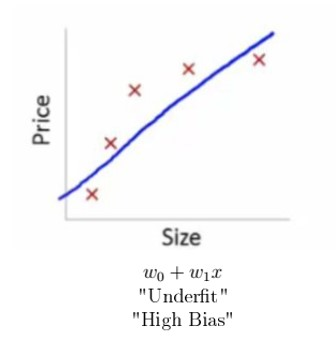
\includegraphics[width=6cm,height=6cm,keepaspectratio]{./pics/HighBias.jpg}
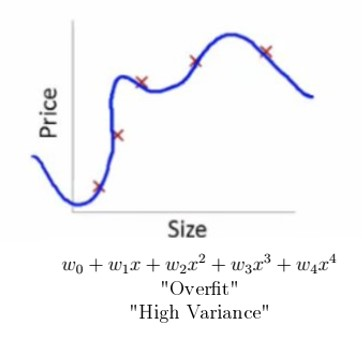
\includegraphics[width=6cm,height=6cm,keepaspectratio]{./pics/HighVariance.jpg}
\end{center}
Nincs elég változó = underfit\\
Túl sok változó = overfit
\newpage
\item Rajzolja fel a tipikus tanító hiba és validációs hiba függvényeket! Jelölje be rajta a "High Bias" és a "High Variance" eseteket!\\
\begin{center}
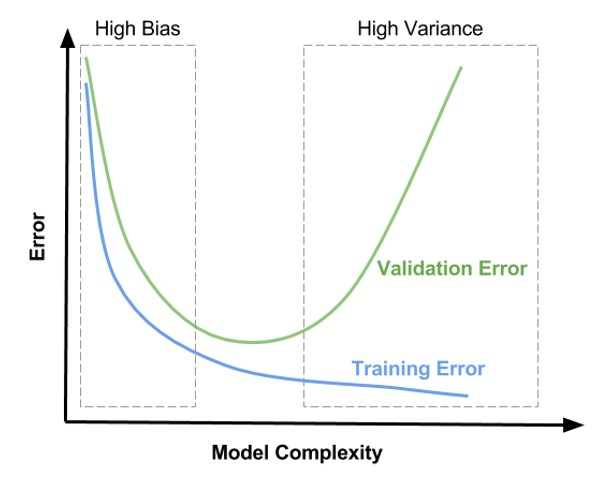
\includegraphics[width=7cm,height=7cm,keepaspectratio]{./pics/TrainValidError.jpg}
\end{center}

\item Mivel lehet kiküszöbölni a "High Bias" és a "High Variance" eseteket?\\
\\
High Variance:\\
- Csökkentjük a változók (featur-ök) számát (kézzel vagy megfelelő modellválasztással.\\
- Több tanító mintát használunk.
- $\lambda$ növelés

High Bias:\\
- Növeljük a változók (featur-ök) számát.(több független változó, polinomiális tagok bevezeteése)\\
- $\lambda$ növelés


Regularizációt vezetünk be (büntetjük a magasabb rendű tagok megjelenését). Így a modell rátanul a megfelelő változókra. A BIAS tagot nem büntetjük!

\newpage
\item Ismertesse a One vs All algortimus működését!\\
\begin{center}
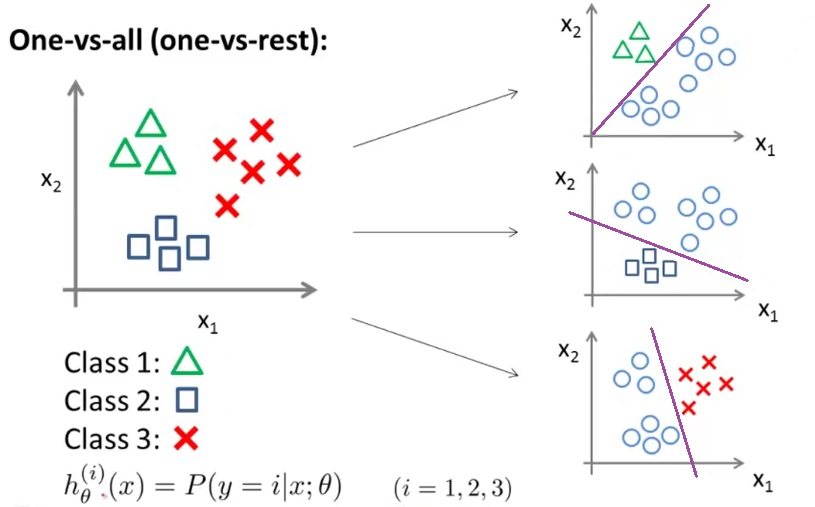
\includegraphics[width=7cm,height=7cm,keepaspectratio]{./pics/OneVsAll.jpg}
\end{center}

\item Rajzolj fel egy előrecsatolt (Fully Connected) neurális hálót ami a következő elemekt tartalmazza: 2 bement, 1 rejtett réteg 3 neuronnal, 1 kimenet! Az ábrán jelöld a súlyokat és írd fel a háló előre lépésének (forward step) alap összefüggéseit!

\begin{center}
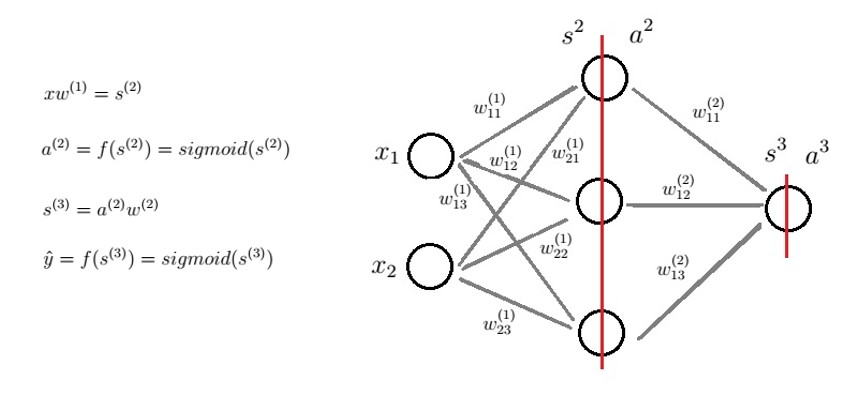
\includegraphics[width=12cm,height=12cm,keepaspectratio]{./pics/ForwardStep.jpg}
\end{center}
\newpage
\item Rajzold fel a szigmoid függvényt és a derivált függvényét jelleghelyesen! Írd fel a képletüket!
\begin{equation}
g(z)=\frac{1}{1+e^{(-z)}}
\end{equation}
\begin{equation}
g'(z)=g(z)\cdot(1-g(z))
\end{equation}
\begin{center}
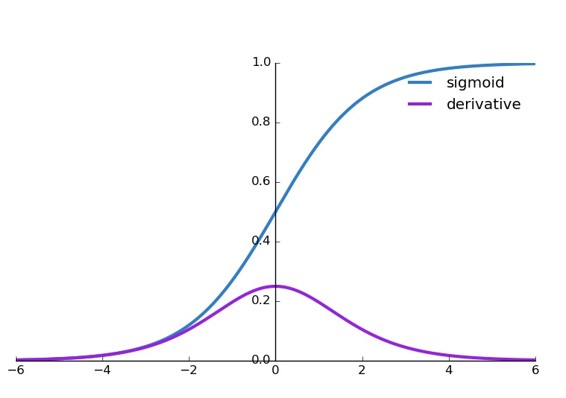
\includegraphics[width=10cm,height=10cm,keepaspectratio]{./pics/sigmoid.jpg}
\end{center}

\item Honnan ismerhető fel, hogy "High Bias" problémával állunk szembe?
\begin{center}
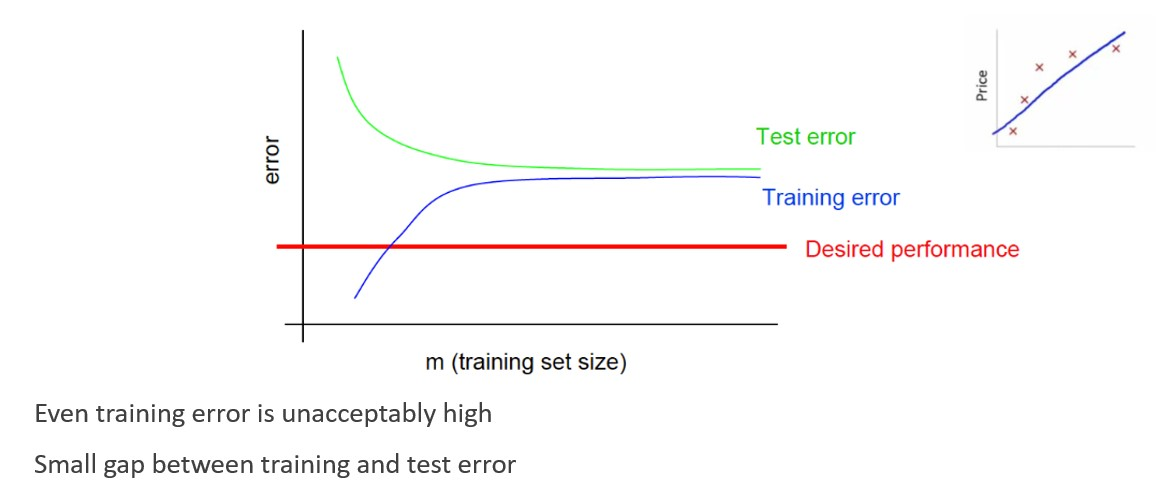
\includegraphics[width=12cm,height=12cm,keepaspectratio]{./pics/ProblemBias.jpg}
\end{center}
\newpage
\item Honnan ismerhető fel, hogy "High Variance" problémával állunk szembe?
\begin{center}
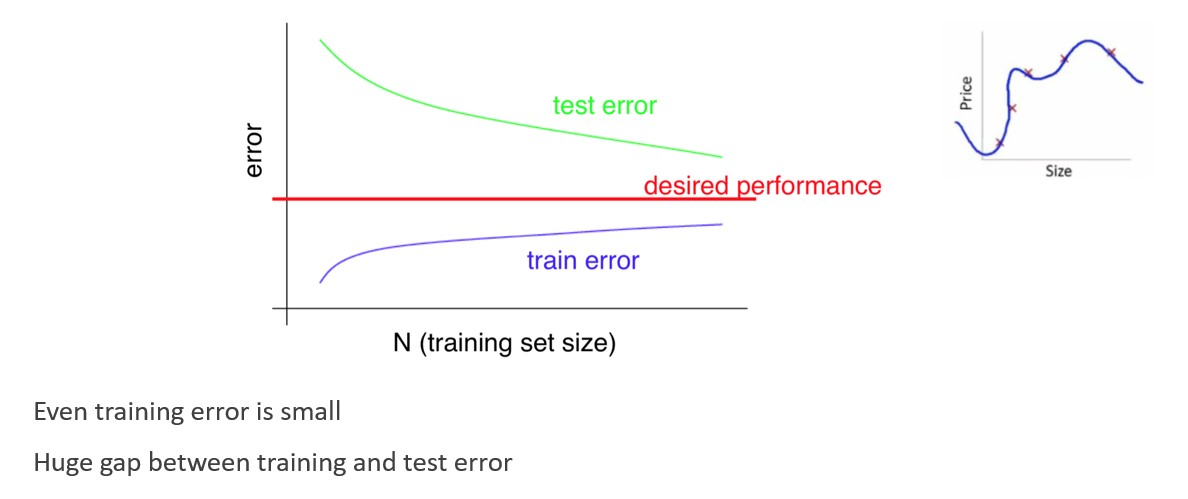
\includegraphics[width=12cm,height=12cm,keepaspectratio]{./pics/ProblemVariance.jpg}
\end{center}

\item Ismertesse az SVM (Support Vector Machine) elvét(ábra)!
\begin{center}
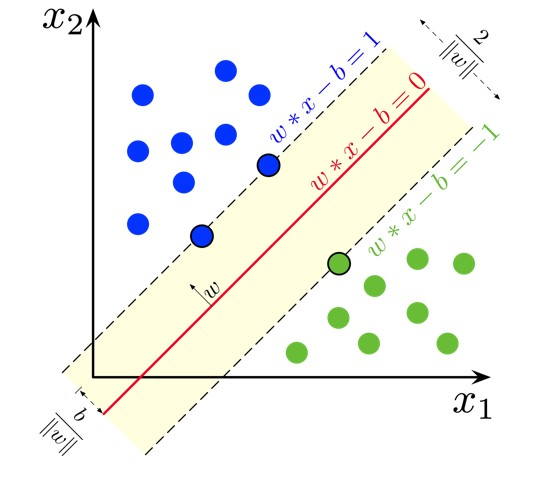
\includegraphics[width=12cm,height=12cm,keepaspectratio]{./pics/SVM.jpg}
\end{center}

\item Spam emailek kategorizálása során milyen előkészítő (normalizáló) lépéseket alkalmazna a bemenetként szolgáló szövegen?\\
\\
- Minden kisbetűs (nagybetűk eltöntetése)\\
- HTML kódrészletek törlése\\
- URL címek helyettesítése taggel.\\
- Email címek helyettesítése taggel.\\
- Számok helyettesítése taggel.\\
- Dollárjel helyettesítés (ezt meg kell tartani)\\
- Szótő redukció\\
- Extra karakterek törlése (*-+/...)\\

\item Ismertesse a K-Means algoritmus működését. (ábra+szöveg)\\
\begin{center}
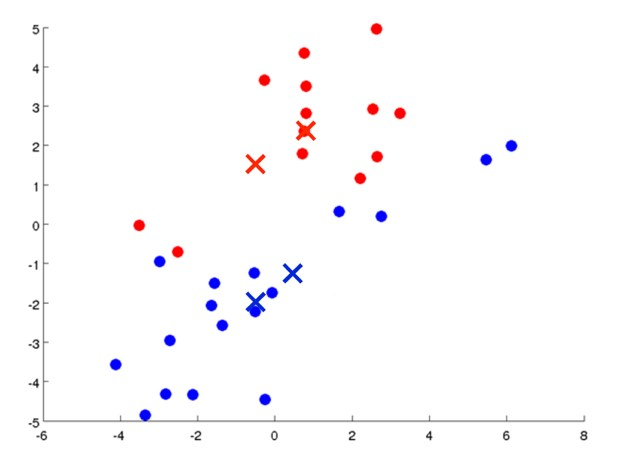
\includegraphics[width=7cm,height=7cm,keepaspectratio]{./pics/KmeansWorking.jpg}
\end{center}
\newpage
\item Mire szolgál a könyök szabály? (ábra)\\
\\
Klaszterek számának meghatározására.\\
\begin{center}
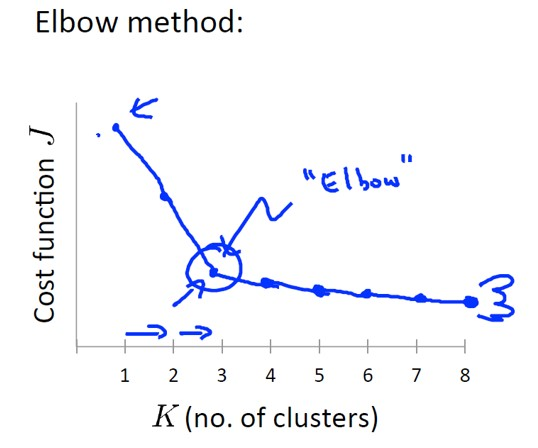
\includegraphics[width=7cm,height=7cm,keepaspectratio]{./pics/ElbowRule.jpg}
\end{center}

\item Ismertesse a PCA (Principal Component Analysis) működését! (ábra+szöveg)
\begin{center}
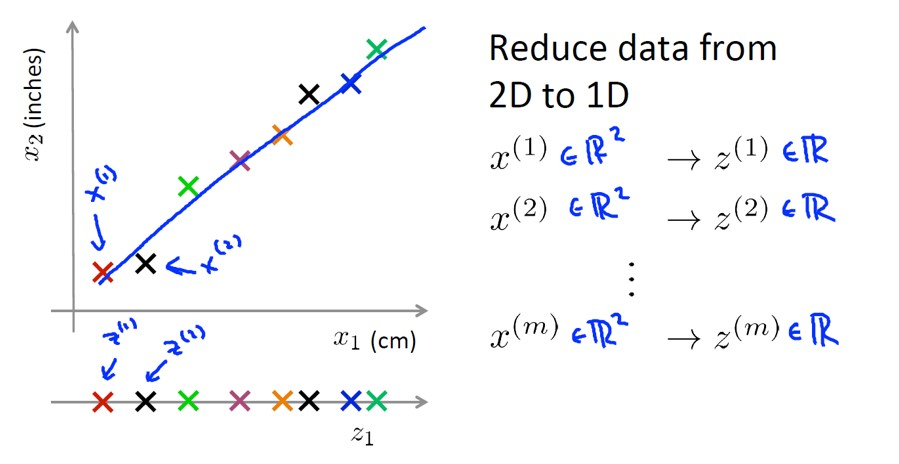
\includegraphics[width=12cm,height=12cm,keepaspectratio]{./pics/PCAworking.jpg}
\end{center}

\end{enumerate}
\end{document}
